Contiene la logica di gioco. 

\begin{itemize}
    \item \textbf{GameState}: rappresenta il mezzo con cui, dall'esterno, ci si può interfacciare con la logica di gioco. Fornisce una serie di funzionalità per gestire la partita, come ad esempio far partire il gioco, chiamare il prossimo step, creare un nuovo livello e gestire i record. All'interno di \textit{GameState} si trova un'istanza della classe \textit{Arena} che rappresenta la mappa di gioco contenente le entità e le varie relazione tra esse.
    
    \item \textbf{MapGenerator}: utilizzato al fine di posizionare nell'ambiente di gioco le proprie entità di partenza come gli ostacoli, i nemici e gli oggetti collezionabili.
    
    \item \textbf{Entity}: come riportato in figura \ref{model}, tutti gli elementi del gioco estendono da questa interfaccia generica. Inoltre  all'entità di base, grazie all'ereditarietà multipla fornita da Scala, si possono decorare le entità con diverse caratteristiche come ad esempio la possibilità di muoversi o di avere una vita. 
\end{itemize}

\begin{figure}[H]
  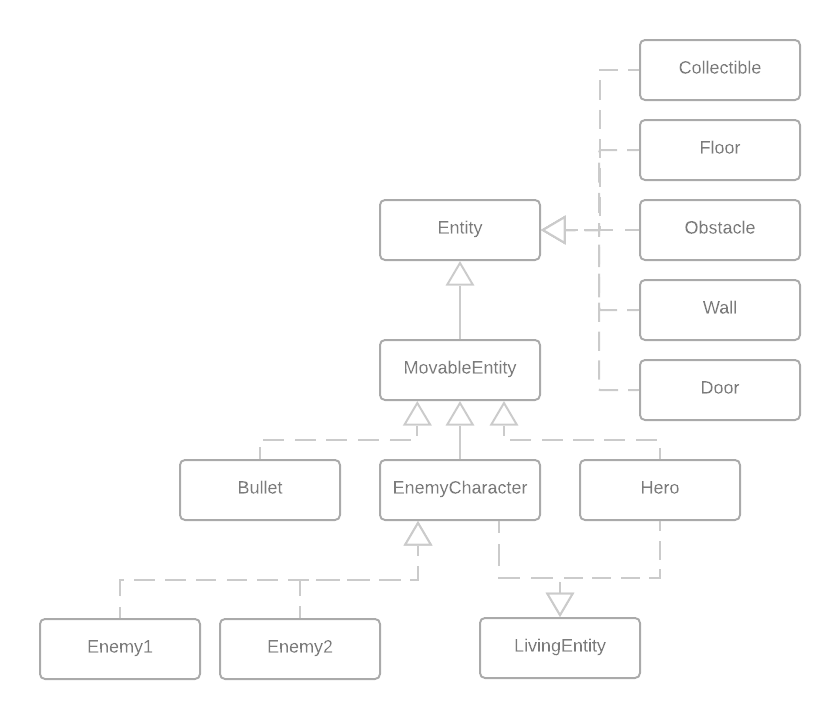
\includegraphics[width=15cm]{report/res/GAMELOGIC_Diagram.png}
  \caption{Organizzazione della logica di gioco}
  \label{model}
\end{figure}